\section{Reconstruction des jets}\label{chapter-JERC-section-jets_reco}
Les particules colorées ne peuvent donc pas être directement observées dans le détecteur.
Leur signature expérimentale est un flux collimé de particules stables composé de hadrons, de leptons et de photons.
La présence de hadrons s'explique directement par le processus de hadronisation décrit dans la section précédente.
Les leptons proviennent de la désintégration, par interaction faible, des hadrons de saveur lourde, ou plus précisément des quarks de deuxième et troisième génération composant ces hadrons lourds.
Les photons sont radiés par les particules électriquement chargées.
\par Un processus physique comme celui de la figure~\ref{subfig-fgraph-Z_q_q} produit seulement quelques particules, en l'occurrence deux, et non des ensembles de particules, comme sur la figure~\ref{fig-agglo_hadronique} qui pourrait correspondre à l'état effectivement observé pour le processus de la figure~\ref{subfig-fgraph-Z_q_q}.
Afin de pouvoir étudier le processus initial, il est nécessaire de définir une observable décrivant les particules colorées à l'origine de ces flux collimés de particules stables.
\par Cette observable est un \og jet \fg.
À partir des particules identifiées à l'aide de l'algorithme de \emph{Particle Flow} (\PF)\footnote{L'algorithme de \emph{Particle Flow} est décrit dans la section~\ifref{chapter-LHC-section-evt_reco-subsec-PF}{\ref{chapter-LHC-section-evt_reco-subsec-PF}}{4.1} du chapitre\ifref{chapter-LHC}{~\ref{chapter-LHC}}{ \og Dispositif expérimental \fg}.}, un algorithme de regroupement permet d'obtenir la liste des jets de l'événement.
Il existe plusieurs algorithmes de regroupement dont le principe est décrit dans la section suivante.
\subsection{Algorithmes de regroupement}\label{chapter-JERC-section-jets_reco-subsec-algo}
Il existe deux catégories d'algorithmes permettant de regrouper les particules en jets, les algorithmes de cônes et les algorithmes de recombinaison séquentielle.
Dans la section~\ref{chapter-JERC-section-jets}, nous avons vu que les radiations de partons sont plus importantes pour de basses énergies (limite infrarouge) ou pour un parton radié colinéaire au parton initial (limite colinéaire).
Afin de conserver des prédictions de QCD vérifiables sur des jets réels, les algorithmes de regroupement doivent être insensibles à l'ajout d'une particule de basse énergie ou au partage d'une particule en deux particules d'énergies inférieures. C'est ce que l'on appelle l'insensibilité IRC, pour \emph{InfraRed and Colinear}.
La plupart des algorithmes de cônes ne sont pas IRC-insensibles, alors que la plupart des algorithmes de recombinaison séquentielle le sont.
\subsubsection{Les algorithmes de cônes}
Les algorithmes de cônes regroupent toutes les particules ayant une direction $\vec{p}$ telle que la distance $\Delta R_{pa}$ à la direction de l'axe du cône $\vec{a}$ dans le plan $(\eta,\phi)$\footnote{Les coordonnées $\eta$ et $\phi$ sont définies dans la section~\ifref{chapter-LHC-section-evt_reco-subsec-PF}{\ref{chapter-LHC-section-CMS-subsec-overview_and_coordinates}}{2.1} du chapitre\ifref{chapter-LHC}{~\ref{chapter-LHC}}{ \og Dispositif expérimental \fg}.} est inférieure à une distance de coupure $R_c$, \ie\ si
\begin{equation}
\Delta R_{pa} ^2 = (\eta_p - \eta_a)^2 + (\phi_p - \phi_a)^2 < R_c^2
\mend
\end{equation}
Alors, la direction $\vec{a}$ du cône et redéfinie comme étant la direction moyenne de toutes les particules rassemblées dans ce cône. Ce processus est itéré jusqu'à la stabilisation des cônes.
Enfin, les cônes sont séparés en cas de superposition, une particule ne pouvant appartenir qu'à un seul jet.
\par L'algorithme \textsc{SISCone}, \emph{Seedless Infrared Safe Cone}, est un exemple d'algorithme de cônes IRC-insensible.
Dans un premier temps, tous les cônes stables possibles sont reconstruits.
Ces cônes sont alors fusionnés, les cônes ayant l'impulsion transverse la plus grande absorbant des cônes d'impulsion transverse moindre dont ils contiennent déjà une fraction.
Un exemple de reconstruction de jets à l'aide de l'algorithme \textsc{SISCone} est présenté sur la figure~\ref{fig-chapter-JERC-section-jets_reco-subsec-algo-examples}.
\subsubsection{Les algorithmes de recombinaison séquentielle}
Les algorithmes de recombinaison séquentielle commencent par considérer que chaque particule forme un jet d'une seule particule.
Puis, à l'aide d'une métrique donnée, la paire de jets les plus proches entre eux fusionne en un seul jet tant que la distance entre eux est en-deçà d'une valeur seuil. Les jets fusionnés donnent la liste des jets de l'événement. Il est également possible de fixer le nombre de jets à déterminer et non la valeur seuil de la distance entre les jets à fusionner.
\par Plusieurs métriques peuvent être définies, chacune correspondant à un algorithme de recombinaison séquentielle proposant des regroupement différents.
\begin{description}
%\item[Algorithme de Durham] La distance $d_{ij}$ entre deux jets $i$ et $j$ est
%\begin{equation}
%d_{ij} = 2 \, \min(E_i^2, E_j^2) \, \frac{1-\cos\theta_{ij}}{Q^2}
%\end{equation}
%où $E_x$ est l'énergie du jet $x$, $\theta_{ij}$ l'angle entre les directions des deux jets et $Q$ l'énergie dans le centre de masse de la collision.
%Cet algorithme a l'avantage de regrouper les particules très fidèlement vis-à-vis de la gerbe hadronique, mais les jets obtenus possèdent une géométrie spatiale irrégulière, comme cela se voit sur la figure~\ref{fig-chapter-JERC-section-jets_reco-subsec-algo-examples}.
\item[Algorithme \kT] La distance $d_{ij}$ entre deux jets $i$ et $j$ est
\begin{equation}
d_{ij} = \min({\pT}_i^2, {\pT}_j^2) \, \frac{\Delta R_{ij}^2}{R^2}
\msep
\Delta R_{ij}^2 = (\eta_i-\eta_j)^2 + (\phi_i-\phi_j)^2
\end{equation}
où ${\pT}_x$ est l'impulsion transverse du jet $x$ et $R$ un paramètre libre.
Cet algorithme a l'avantage de regrouper les particules très fidèlement vis-à-vis de la gerbe hadronique, mais les jets obtenus possèdent une géométrie spatiale irrégulière, comme cela se voit sur la figure~\ref{fig-chapter-JERC-section-jets_reco-subsec-algo-examples}.
\item[Algorithme de Cambridge/Aachen] La distance $d_{ij}$ entre deux jets $i$ et $j$ est
\begin{equation}
d_{ij} = \frac{\Delta R_{ij}^2}{R^2}
\msep
\Delta R_{ij}^2 = (\eta_i-\eta_j)^2 + (\phi_i-\phi_j)^2
\end{equation}
où $R$ est un paramètre libre. Le regroupement des jets est ainsi uniquement basé sur l'écart angulaire.
\item[Algorithme anti-\kT~\cite{Cacciari_antikT}] La distance $d_{ij}$ entre deux jets $i$ et $j$ est
\begin{equation}
d_{ij} = \min\left(\frac{1}{{\pT}_i^2}, \frac{1}{{\pT}_j^2}\right) \, \frac{\Delta R_{ij}^2}{R^2}
\msep
\Delta R_{ij}^2 = (\eta_i-\eta_j)^2 + (\phi_i-\phi_j)^2
\end{equation}
où ${\pT}_x$ est l'impulsion transverse du jet $x$ et $R$ un paramètre libre.
Le regroupement des particules se fait ainsi autour des particules de plus haute énergie.
Cet algorithme propose un regroupement des particules moins fidèle à la gerbe hadronique, mais produit des jets de forme régulière, comme cela se voit sur la figure~\ref{fig-chapter-JERC-section-jets_reco-subsec-algo-examples}.
\end{description}
\begin{figure}[h]
\centering
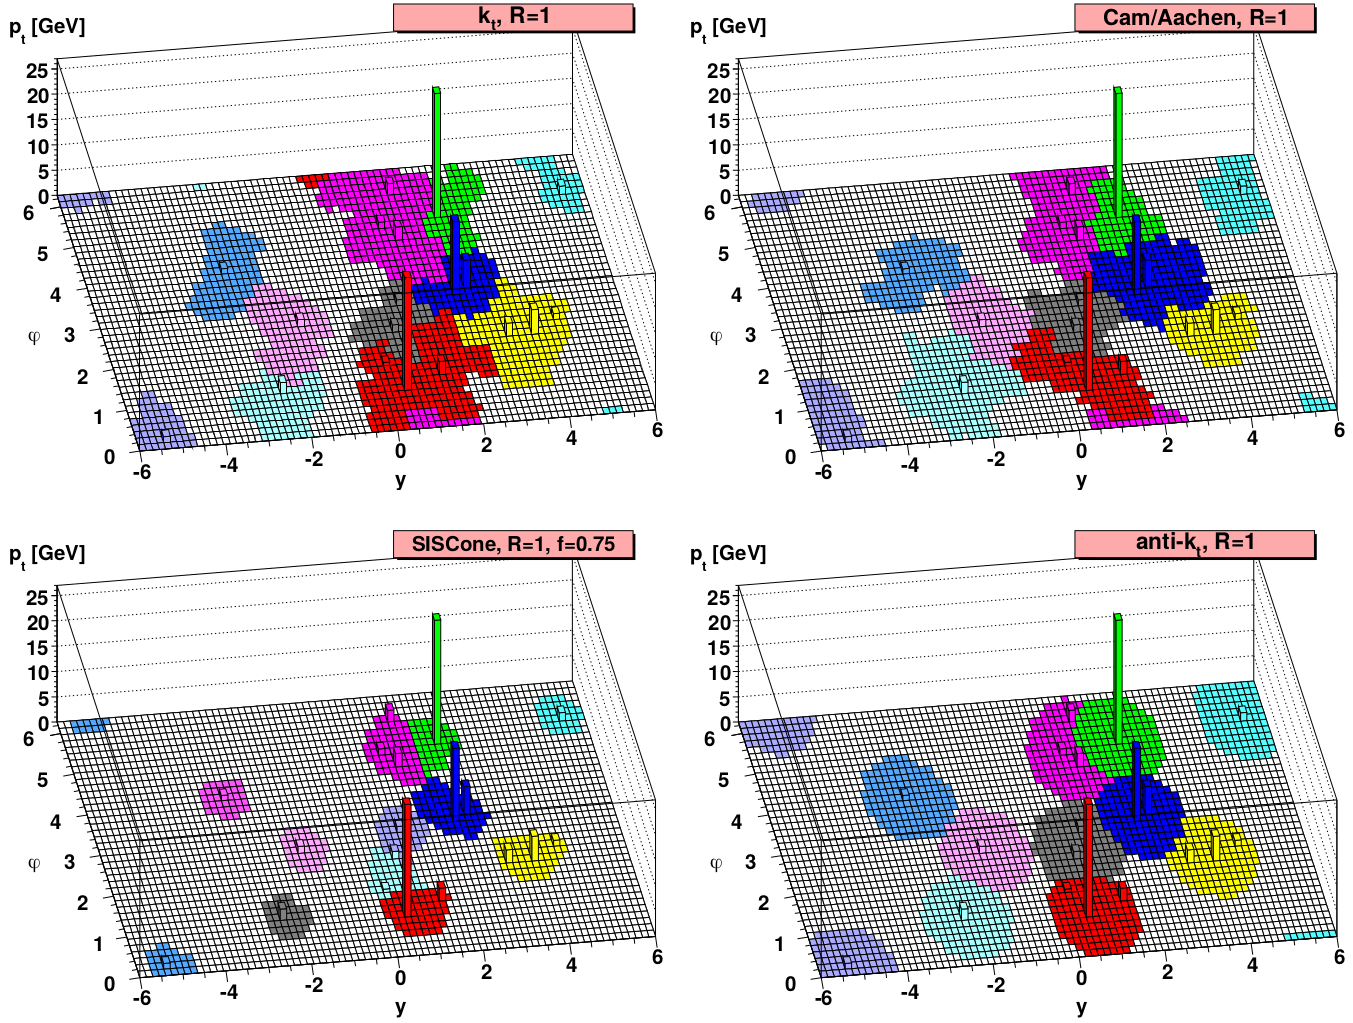
\includegraphics[width=.8\textwidth]{\PhDthesisdir/contents/chapter-JERC/reconstruction_des_jets/forme_des_jets.png}
\caption{Formes des jets reconstruits à partir de différents algorithmes pour un même événement. En haut à gauche, \kT; en haut à droite, C/A; en bas à gauche, \textsc{SISCone}; en bas à droite, anti-\kT. L'algorithme anti-\kT\ permet d'obtenir des jets de forme régulière, conique.}
\label{fig-chapter-JERC-section-jets_reco-subsec-algo-examples}
\end{figure}


\begin{figure}
\centering
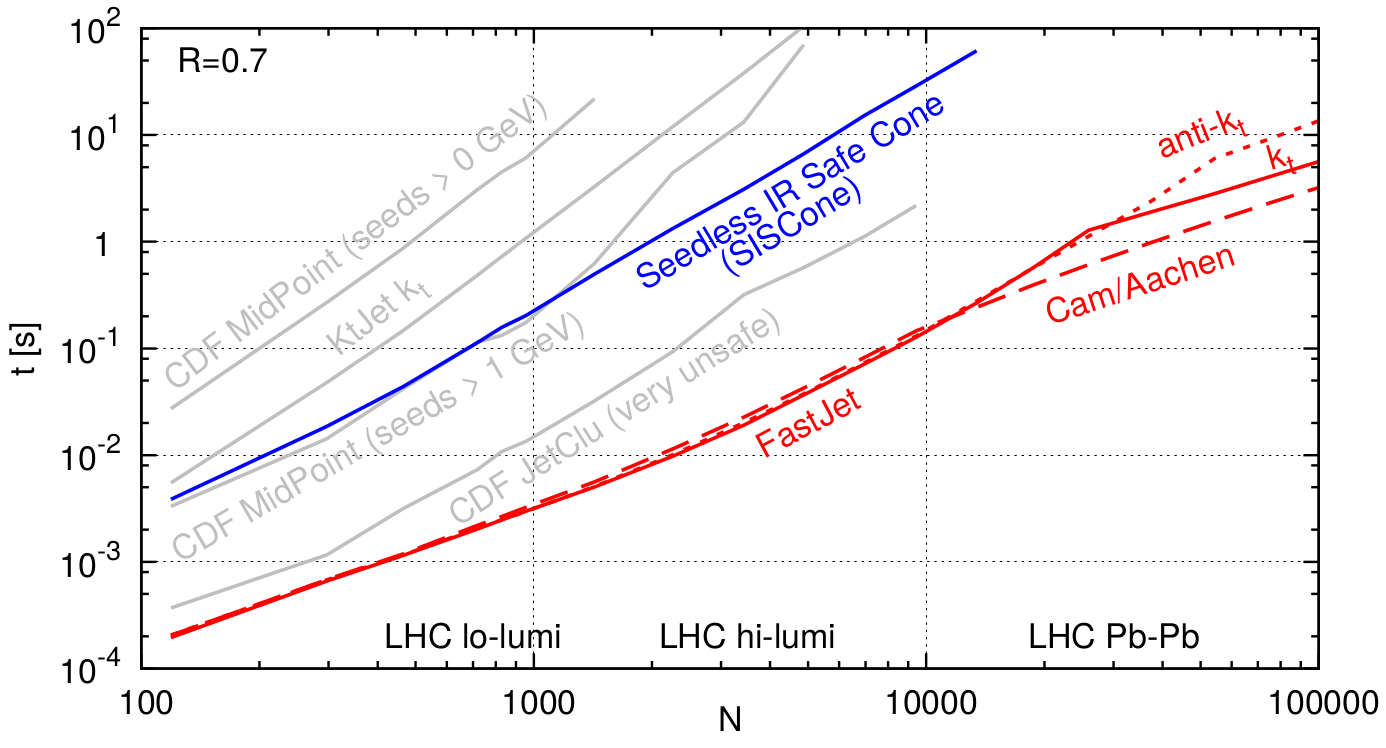
\includegraphics[width=.6\textwidth]{\PhDthesisdir/contents/chapter-JERC/reconstruction_des_jets/temps_de_calcul.png}
\caption{Temps de reconstruction d'un empilement d'un événement di-jets avec $N$ événements ne produisant que des jets de bas \pT\ pour différents algorithmes de reconstruction des jets.} % 50 GeV
\end{figure}

\subsection{Identification des jets dans CMS}\label{chapter-JERC-section-jets_reco-subsec-jetID}
quels critères?

\subsection{Saveur des jets}\label{chapter-JERC-section-jets_reco-subsec-flavor}
b-tagging

\begin{figure}
\centering
\begin{tikzpicture}[scale=1.5]
\def\trackerrin{.100}
\def\trackerrout{1.185}
\def\trackercolor{ltcolorgray1}

\def\ECALrin{1.290}
\def\ECALrout{1.811}
\def\ECALcolor{ltcolorgreen1}

\def\HCALrin{1.812}
\def\HCALrout{2.854}
\def\HCALcolor{ltcoloryellow3}

\def\Solenrin{2.950}
\def\Solenrout{3.800}
\def\Solencolor{ltcolorgray2}

\def\ironryrina{3.850}
\def\ironryrouta{4.000}
\def\muonrina{4.020}
\def\muonrouta{4.400}
\def\ironryrinb{4.420}
\def\ironryroutb{4.880}
\def\muonrinb{4.905}
\def\muonroutb{5.285}
\def\ironryrinc{5.300}
\def\ironryroutc{5.960}
\def\muonrinc{5.975}
\def\muonroutc{6.355}
\def\ironryrind{6.375}
\def\ironryroutd{6.980}
\def\muonrind{7.000}
\def\muonroutd{7.380}
\def\muoncolor{ltcoloryellow1}
\def\ironrycolor{ltcolorred2}

\def\printele#1{
\draw [thick, ltcolorred] (0,0) arc (#1-90:#1-90+27:3) coordinate (eledeposit);
\draw [ltcolorred] (#1-5:1.25) node {\ele};
}
\def\printmu#1{
\draw [thick, ltcolorblue] (0,0) arc (#1-90:#1-90+33:6) arc (#1-90+33:#1-90:-12) node{\mu};
\draw [ltcolorblue] (#1-7:1.5) node {\mu};
}

\def\printantiele#1{
\draw [thick, ltcolorred] (0,0) arc (#1-90:#1-90-27:-3) coordinate (eledeposit);
\draw [ltcolorred] (#1-7:1.5) node {\ele};
%\draw [ltcolorred4, ultra thick] (eledeposit)--+(#1+25:\ECALrout);
}
\def\printantimu#1{
\draw [thick, ltcolorblue] (0,0) arc (#1-90:#1-90-33:-6) arc (#1-90-33:#1-90:12);
\draw [ltcolorblue] (#1-7:1.5) node {\mu};
}

\def\printtauh#1{
\draw [thick, ltcolorgreen4] (0,0) arc (#1-90:#1-90+11:10) ;
\draw [thick, ltcolorgreen4] (0,0) arc (#1-90:#1-90+6:20) ;
\draw [thick, ltcolorgreen4] (0,0) arc (#1-90:#1-90-11:-10) ;
\draw [ltcolorgreen4] (#1-12:1.5) node {\tauh};
}
\def\printantitauh#1{
\draw [thick, ltcolorgreen4] (0,0) arc (#1-90:#1-90-11:-10) ;
\draw [thick, ltcolorgreen4] (0,0) arc (#1-90:#1-90-6:-20) ;
\draw [thick, ltcolorgreen4] (0,0) arc (#1-90:#1-90+11:10) ;
\draw [ltcolorgreen4] (#1-12:1.5) node {\tauh};
}

\def\printjetnolabel#1{
\draw [thick, ltcolororange] (0,0) arc (#1-90+10:#1-90+22+10:5) ;
\draw [thick, ltcolororange] (0,0) arc (#1-90+5:#1-90+12+5:10) ;
\draw [thick, ltcolororange] (0,0) arc (#1-90:#1-90-22:-5) ;
\draw [thick, ltcolororange] (0,0) arc (#1-90:#1-90+6:20) ;
\draw [thick, ltcolororange] (0,0) arc (#1-90+5:#1-90+8+5:10) ;
\draw [thick, ltcolororange] (0,0) arc (#1-90:#1-90-11:-10) ;
\draw [thick, ltcolororange] (0,0) arc (#1-90:#1-90+11:10) ;
}

\def\printjet#1{
\printjetnolabel{#1}
\draw [ltcolororange] (#1-25:.5) node {jet};
}

\def\printjetfake#1{
\printjet{#1}
\draw [thick, ltcolorgreen4] (0,0) arc (#1-90:#1-90+11:10) ;
\draw [thick, ltcolorgreen4] (0,0) arc (#1-90:#1-90+6:20) ;
\draw [thick, ltcolorgreen4] (0,0) arc (#1-90:#1-90-11:-10) ;
\draw [ltcolorgreen4] (#1-17:1.5) node {f.\tauh};
}

\def\printdeposit#1#2#3#4{
\fill [#1] (#2-2:#3) arc (#2-2:#2+2:#3) -- (#2+2:#4) arc (#2+2:#2-2:#4) ;
}

\def\printECALdeposit#1#2{\printdeposit{#1}{#2}{\ECALrin}{\ECALrout}}
\def\printHCALdeposit#1#2{\printdeposit{#1}{#2}{\HCALrin}{\HCALrout}}

\def\printtauhdeposit#1{
\printHCALdeposit{ltcoloryellow4}{#1+3}
\printHCALdeposit{ltcoloryellow4}{#1+5}
\printHCALdeposit{ltcoloryellow4}{#1-5}
}

\def\printjetdeposit#1{
\printHCALdeposit{ltcoloryellow4}{#1+3}
\printHCALdeposit{ltcoloryellow4}{#1+5}
\printHCALdeposit{ltcoloryellow4}{#1-5}
\printHCALdeposit{ltcoloryellow4}{#1+21}
\printHCALdeposit{ltcoloryellow4}{#1+11}
\printHCALdeposit{ltcoloryellow4}{#1-11}
}

\def\printMuChSigA#1#2{
\fill [red] (#1-7.5+20*#2:\muonrina) arc (#1-7.5+20*#2:#1+7.5+20*#2:\muonrina) -- (#1+7.5+20*#2:\muonrouta) arc (#1+7.5+20*#2:#1-7.5+20*#2:\muonrouta) ;
}
\def\printMuChSigB#1#2{
\fill [red] (#1-7.5+20*#2:\muonrinb) arc (#1-7.5+20*#2:#1+7.5+20*#2:\muonrinb) -- (#1+7.5+20*#2:\muonroutb) arc (#1+7.5+20*#2:#1-7.5+20*#2:\muonroutb) ;
}
\def\printMuChSigC#1#2{
\fill [red] (#1-7.5+20*#2:\muonrinc) arc (#1-7.5+20*#2:#1+7.5+20*#2:\muonrinc) -- (#1+7.5+20*#2:\muonroutc) arc (#1+7.5+20*#2:#1-7.5+20*#2:\muonroutc) ;
}
\def\printMuChSigD#1#2{
\fill [red] (#1-7.5+20*#2:\muonrind) arc (#1-7.5+20*#2:#1+7.5+20*#2:\muonrind) -- (#1+7.5+20*#2:\muonroutd) arc (#1+7.5+20*#2:#1-7.5+20*#2:\muonroutd) ;
}

\foreach\jetangle in {120,-145}{
\printbigjetnolabel{\jetangle}
\draw (\jetangle:2.5) node {jet} ;
}

\def\Bjetangle{30}
\def\Bhaddronangle{5}
\def\Bhaddronflight{.75}

\def\CurrentVertex{(\Bhaddronangle:\Bhaddronflight)}

\draw [thick, dotted] (0,0) -- \CurrentVertex ;

{
\def\jetcolor{ltcolorred}
\printjetnolabel{\Bjetangle}
\draw [\jetcolor] (\Bjetangle:2)+(1.5,.75) node {traces déplacées};
}
\begin{scope}
\clip circle (\Solenrin);
\printantimuonnolabel{\Bjetangle}
\end{scope}

\draw [\muoncolor] (\Bjetangle:4) +(0,{-2*\baselineskip}) node {lepton chargé};

\draw (\Bjetangle:4) + (-.125,-.5) circle (1.125);
\draw [-latex] (\Bjetangle:4) + (-.125,-1.625) --+ (-.125,-2) node [below] {jet de saveur lourde};

\draw (0,0) node [left] {PV} ;
\draw \CurrentVertex node [below right] {SV} ;

\fill (0,0) circle (2pt);
\fill \CurrentVertex circle (2pt);

\draw [dashed] \CurrentVertex --+ (\Bjetangle:-.8);

\draw [red, latex-latex] (0,0)--+ (-90+\Bjetangle:{\Bhaddronflight*sin(\Bjetangle-\Bhaddronangle)}) node [below right] {IP};
\end{tikzpicture}
\end{figure}